\usetikzlibrary{chains, calc}
\begin{document}
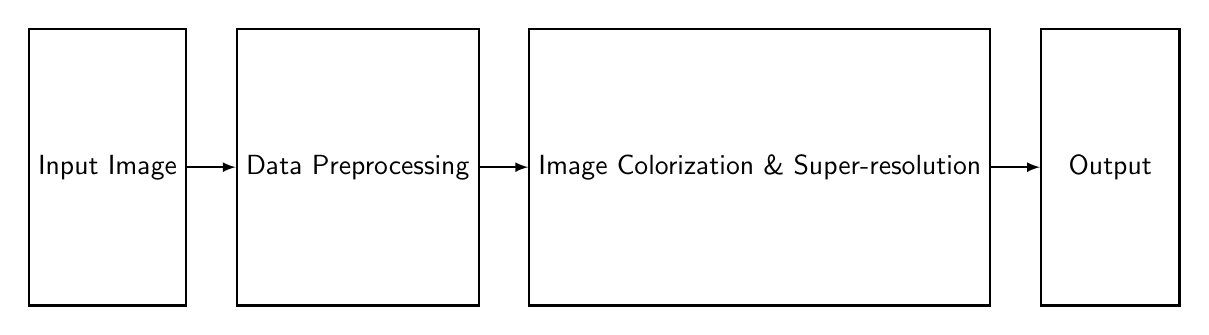
\begin{tikzpicture}[box/.style={draw,thick,minimum width=5em,minimum
    height=10em},arj/.style={semithick,-latex}]
  \begin{scope}[start chain=A going right,oc/.style={join=by arj,on chain},
    font=\sffamily,node distance=1.75em]
   \node(input)[box,oc]{Input Image};
   \node[box,oc]{Data Preprocessing};
   \node[box,oc]{Image Colorization \& Super-resolution};
   \node[box,oc]{Output};
  \end{scope}
\end{tikzpicture}